\chapter{Introduction}
\label{chap:intro}


\section{Introduction}

The classic problem about vehicle routing (VRP) is an well known \textit{NP-hard} ~\cite{Lenstra_1981} optimization problem of importance in different logistics, it consist in delivery goods to a set of costumers geographically dispersed, using a fleet of vehicles that begin its route in the central depot. The problem consists in to assign to each vehicle a route with the objective of minimizing the transportation cost.

The cost generated in the transport of goods, like the size of the fleet of vehicles maintenance, combustible, and so on, are significant owing to the transport processes are involved at all stages of production processes, accounting for 10\% to 20\% of the final product cost~\cite{toth_vehicle_2001}.

One of the first investigation that studied the vehicle routing problem was in the year 1959, in that work Dantzing and Ramser~\cite{Dantzing1959} analyzed an oil dispatching problem with trucks, that problem arise as a generalization of the classic traveling salesman problem (TSP), where the salesman has to visit a set of costumers only one time, and then come back to the origin point, building a Hamiltonian road on the graph consisting of customers (vertices) and the possible paths between clients (edges).

Different variations of the VRP have been proposed with the aim of approaching the problem real contexts; these problems include the addition of variables and constraints. The figure below shows a diagram with the most popular variants of VRP.

\begin{figure}[!htbp]
  \begin{center}
    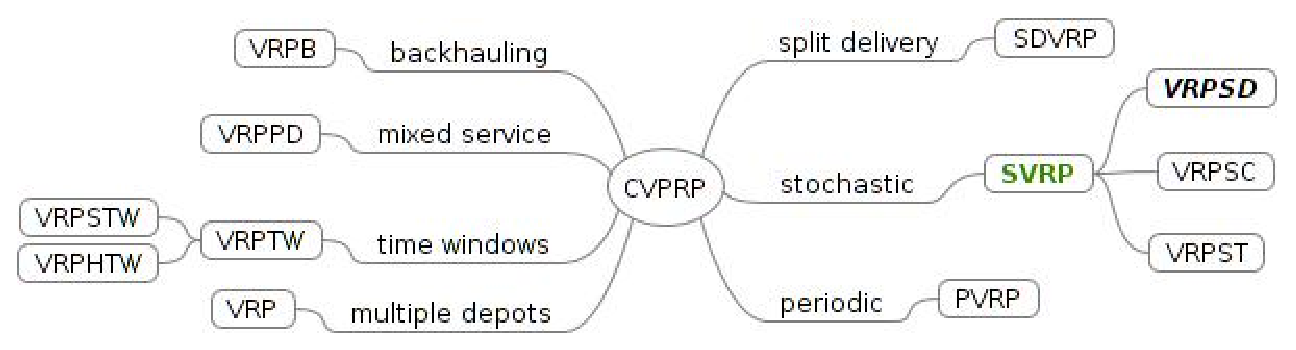
\includegraphics[width=0.8\textwidth]{Images/Chapter1/variants_vrp.eps}
  \end{center}
  \caption{Basic variants of the Vehicle Routing Problem}
  \label{fig:VRP_variants}
\end{figure}

When vehicles capacity is fixed origin the CVRP (Capacited Vehicle Routing Problem); if there are many depots, then we have MDVRP (Multiple Deposit Vehicle Routing Problem). The SDVRP (Split delivery Vehicle routing problem) is a relaxation of the problem that allows a costumer be served by several vehicles, being important in cases where the customer demand exceeds the vehicle capacity. Generally the VRP provide a planning for a fixed period, the PVRP (Periodic Vehicle Routing Problem) provides that planning for $m$ periods.

One of the most studied variants of the problem is caused by including time windows for deliveries, VRPTW (Vehicle Routing Problem with Time Windows), for this problem can be considered hard time windows (VRTHTW) that can't be done delivery outside the established periods, and soft time windows (VRPSTW) in which deliveries can be made outside these periods with a penalty.

The problems that include pick-up and delivery can be divided in VRPB (Vehicle Routing Problem with Backhauls) and VRPPD (Vehicle Routing Problem with Pick-Up and Delivery) in the VRPB the group of costumers is divided in two subgroups, for the first group all pick-up's are made of some product, then the vehicle return to the depot, then the deliveries are realized to the second group of costumers.  In the VRPPD the pick-up's and deliveries to customers are made simultaneously.

The SVRP (Stochastic vehicle routing problem) arise when there is uncertainty about some of the components of the VRP, i.e. one or more variables are random, usually these problems include VRPSC (Vehicle routing problem with stochastic costumers) that include random customers, the VRPST (Vehicle Routing Problem with Stochastic Times) where travel times are random and VRPSD (Vehicle Routing Problem with Stochastic Demands), where the customers' demands are known only with a probability distribution.

The SVRP's differ from the deterministic VRP in many important aspects. The solution concept is different, many properties of the deterministic problem are not manageable in the stochastic case and solution methodologies are considerably more complex, often SVRP is considered a computationally intractable problem and only small instances can be solved optimally and algorithms are difficult to design and evaluate~\cite{gendreau_stochastic_1996}.

The SVRP is either often modeled in the framework of stochastic programming (optimization) integer or mixed or as a Markov decision process. In stochastic programming, problems are usually modeled as two-stage usually as chance constrained program (CCP) or as a stochastic program with recourse (SPR).

The VRPSD is an open problem of great importance in logistics owing to the diversity of real situations it represents, this problem occur in the delivery of home heating oil~\cite{dror_computational_1985} in which each customer maintains a local inventory of the product and consumes a amount of oil each day, therefore each day a fleet of trucks is dispatched to resupply a subset of customers, stochastic demands are also evident in the collection of money by the vehicles of values, e.g. is touched off when collect money by a central bank~\cite{jianhua_fan_multiple_2006} from several but not all of its branches every day, the capacity of the vehicle used may be constrained for an upper bound on the amount of money that a vehicle might carry for safety reasons. The distribution of demand at each certain branch may be different, associated with the amount of money it handles. Other VRPSD arise in delivering the post to large customers~\cite{Markovic_2005}, vending machines~\cite{yang_stochastic_2000} or delivering medical supplies in response to large-scale emergency~\cite{dessouky_rapid_2006}, in recycling and waste management, among others.

\section{Proposal}

Design a hybrid evolutionary algorithm which combine stochastic dynamic optimization operators to find solutions for the vehicle routing problem with stochastic demands, moreover evaluate the algorithm performance.


\section{Objective}

Design and test a hybrid evolutionary algorithm + stochastic dynamic optimization (SDO) operators for the vehicle routing problem with stochastic demands.

\subsection{Specifics Objectives}

\begin{enumerate}
 \item Analyze the alternatives for modeling and representing problem, and selected the most computationally convenient.
 \item Design evolutionary and stochastic dynamic optimization operators algorithm to solve VRPSD.
 \item Implement the designed algorithm.
 \item Select benchmarking problems instances and alternative algorithms for testing.
 \item Develop experimental analyses and comparisons.
\end{enumerate}

\section{Contributions}

The evolutionary algorithms haven't been broadly used to solve the vehicle routing problem with stochastic demands, thus a hybrid evolutionary algorithm which combine stochastic dynamic optimization operators is proposed, it contribute with a new methodology to deal with the problem.

\section{Outline}

In this first chapter was carried out a summary of the issues to be addressed, in chapter 2 presents the background and is presented the state of the art of the VRPSD, chapter 3 presents the Methodology used and presents the proposed algorithm, the chapter 4 presents the experiments, the numerical results and compare and discuss the results comparing with the outcomes obtained by other authors, finally in chapter 5 presents the conclusions of the study.

